\chapter{Information Visualisation aspects}
\label{chapter:iv}
In this chapter, we describe all the choices and aspects of the application related to the purpose of the course which is the Information Visualisation. We also cover a part of User Experience.

%-------------------------------------------------------------------------------
%-------------------------------------------------------------------------------
\section{Target audience}
This app is provided to different financial actors, from analysts, to managers and even students. It helps the user to create a mental model bringing together what were the stocks values at some time and what appeared in the news around this event, which might lead to be an answer and to understand the evolution of the price.

%-------------------------------------------------------------------------------
%-------------------------------------------------------------------------------
\section{Data to visualize}
The first question to ask is what is the data we are using and what information we want to give to the user. As stated in section~\ref{sec:intro:features}, we want to give a clear picture of the different events that occured within a specific range of time (e.g. 1 year) by providing news related to the events.
For example, if the shared stock value of some company dropped on 3$^{\text{rd}}$ July 2015, the user might want to know what happened on this particular day. Thus, the app will retrieve the news that talk about the company around that day. Maybe that an article from \textit{Reuters} or \textit{Swissquote} will explain why the shared stock value lost 50 \$.

The data is numerical, quantitative and temporal (i.e. expressed with a time dimension). Defaults are set to present 1 year from the current day of stock values, 5 events occuring in this time frame, and the articles in a range of 2 months before and after the event.

In the next sections, we are describing more precisely the different information present on the app and how we decided to represent them.

%-------------------------------------------------------------------------------
\subsection{Stock values}
To represent the stock values we used a chart created with the Javascript library HighchartsJS, or more specifically, with HighstocksJS, a library using HighchartsJS. In the figure~\ref{fig:stockchart}, we see Facebook (FB) stock prices in a one year time range.
\begin{figure}
    \centering
    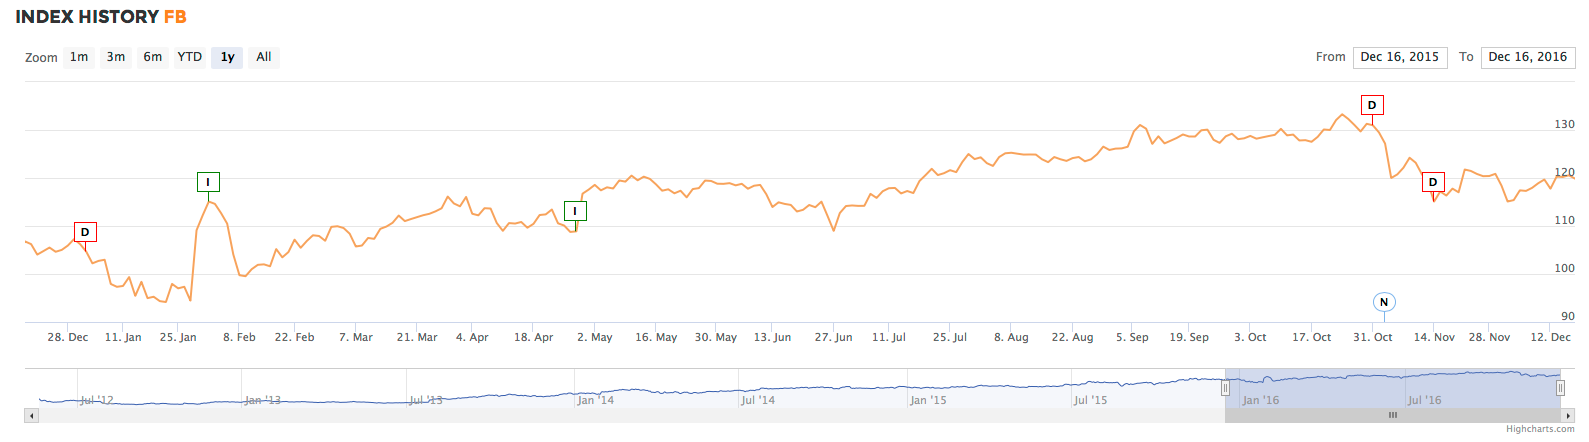
\includegraphics[scale=0.24]{Figures/stock-values.png}
    \caption{Example of visualisation of the Facebook (FB) stock price between the 16$^{\text{th}}$ December 2015 and 16$^{\text{th}}$ December 2016.}
    \label{fig:stockchart}
\end{figure}
There are two important visual enhancements to a simple line chart present in our chart. First, there are two visualization of the data itself, one big of current timeframe and a second one smaller below the big one representing briefly the whole data set. And secondly, the different events were added as flags on the line to let the user visualize at first sight when the events occured. The flags are here to amplify cognition.

In addition of the visual enhancements, there is also the possibility to interact directly with the chart and zoom to a particular range or to drag the mouse and know what we are pointing at.

As our target is financial actors, representing the line chart is what they are used to when they look at the evolution of the stock price. Thus, in order to be the least surprising to them, we decided to also use a line chart.

%-------------------------------------------------------------------------------
\subsection{Events}
Before getting at how we represented the events, let us define what an event is.
\begin{center}
    An event is understood as a ``\textit{significant decrease or increase in a short amount of time}''.
\end{center}
An event is linked to the information provided by the line chart. In order to keep this temporal dimension, we decided to represent the events on a non-scaled (i.e. the separation between the dates does not respect the actual time difference) timeline. The timeline is top-bottom, which means that the most recent event is at the top and the others follow in a reversed chronological order.

Besides the time information, we also represent the type of event. Is it an event due to a significant increase (i.e. positive event) or decrease (i.e. negative event)? To answer this question, let us consider the figure~\ref{fig:event-timeline}. An arrow facing up describes a positive event and, \textit{a contrario}, an arrow facing down describes a negative event. This information is amplified by the color. A green or red arrow is used for respectively a positive or a negative event.

The highlighted event helps the user to reminder what event is currently used to retrieve the news.

% TODO Correct the text on the figure

\begin{figure}
    \centering
    % 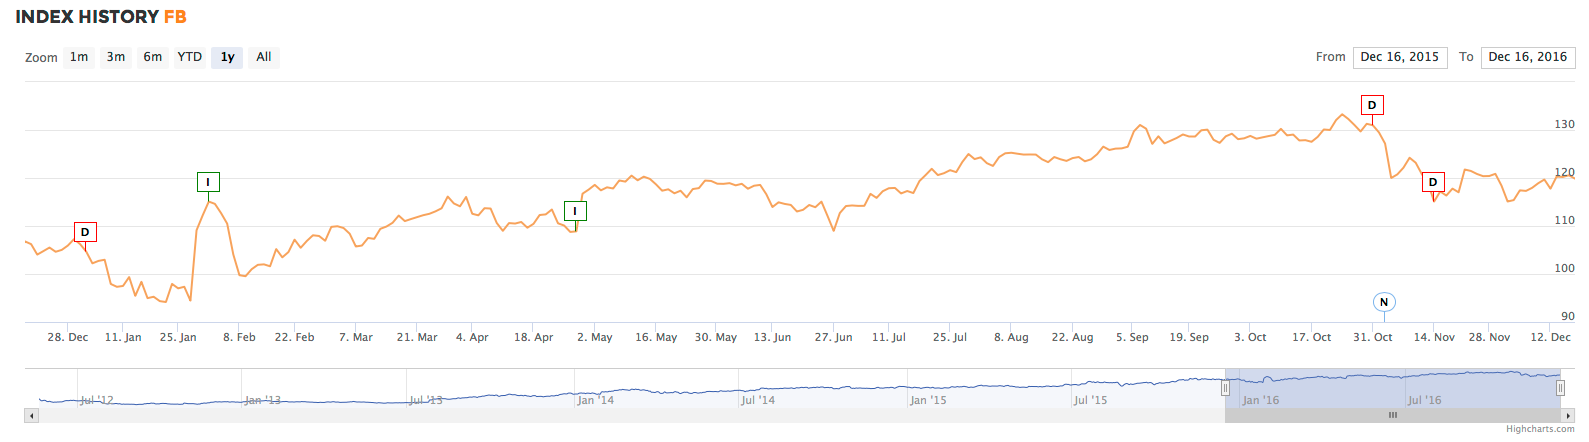
\includegraphics[scale=0.24]{Figures/stock-values.png}
    \textbf{Here add the screenshot of the timeline of events}
    \caption{Example of visualisation of the Facebook (FB) stock price events between the 16$^{\text{th}}$ December 2015 and 16$^{\text{th}}$ December 2016.}
    \label{fig:event-timeline}
\end{figure}

%-------------------------------------------------------------------------------
\subsection{News}
simple list with highlights

%-------------------------------------------------------------------------------
%-------------------------------------------------------------------------------
\section{One page design}
why one page design
why chart left + timeline right => eyes path

%-------------------------------------------------------------------------------
%-------------------------------------------------------------------------------
\section{The orange color}
As shown in the third lecture\footnote{InfoVisMSE\_03.pdf, p.13} of the course, a different color helps the perception as a \textit{preattentive processing}, for example to highlight information. In our case, what we are highlighting is the data that changes through the use of the application. Here is the list of orange representation on the application.
\begin{itemize}
    \item Line in the chart
    \item Current index
    \item Events range
    \item News relevant to an event
\end{itemize}
The purpose is to catch the eye when the user does not remember the context of what he is looking at and needs a refresh.

%-------------------------------------------------------------------------------
%-------------------------------------------------------------------------------
\section{User Experience}
one page design
loading spinkits
interactions: explore (stocks options value, news), reconfigure (events on timeline, events as flags on chart), abstract / elaborate (change date range), connect (select a range changes the events, select an event changes the news)
tasks: overview, zoom, detail on demand, history

%-------------------------------------------------------------------------------
%-------------------------------------------------------------------------------
\section{Easter egg}
This is a secret section. However, if you gently ask a Storm Trooper, he might reveal it.
